% ****** Start of file aipsamp.tex ******
%
%   This file is part of the AIP files in the AIP distribution for REVTeX 4.
%   Version 4.1 of REVTeX, October 2009
%
%   Copyright (c) 2009 American Institute of Physics.
%
%   See the AIP README file for restrictions and more information.
%
% TeX'ing this file requires that you have AMS-LaTeX 2.0 installed
% as well as the rest of the prerequisites for REVTeX 4.
%
% It also requires running BibTeX. The commands are as follows:
%
%  1)  latex  aipsamp
%  2)  bibtex aipsamp
%  3)  latex  aipsamp
%  4)  latex  aipsamp
%
% Use this file as a source of example code for your aip document.
% Use the file aiptemplate.tex as a template for your document.
\documentclass[%
aip,
%jmp,%
%bmf,%
%sd,%
rsi,%
 amsmath,amssymb,%floatfix,
%preprint,%
 reprint,%
%author-year,%
%author-numerical,%
]{revtex4-1}

\usepackage{graphicx}% Include figure files
\usepackage{dcolumn}% Align table columns on decimal point
\usepackage{bm}% bold math
%\usepackage[mathlines]{lineno}% Enable numbering of text and display math
%\linenumbers\relax % Commence numbering lines

%\usepackage{caption}
%\usepackage{subcaption}
\usepackage{cleveref}

\begin{document}

\preprint{AIP/123-QED}

\title[Sample title]{Evidence of terbium and oxygen co-segregation in annealed AlN:Tb}% Force line breaks with \\
%\thanks{Footnote to title of article.}

\author{V.C. Angadi}
\email[e-mail: ]{vcangadi1@sheffield.ac.uk}

\author{T. Walther}%
\email[e-mail: ]{t.walther@sheffield.ac.uk}

\affiliation{Dept. Electronic \& Electrical Eng., Kroto Centre for High-Resolution Imaging and Spectroscopy, University of Sheffield, North Campus, Wheeldon Street, Sheffield S3 7HQ, UK}

\author{F. Benz}
\affiliation{Institute of Materials Science, University of Stuttgart, Heisenbergstr. 3, 70569 Stuttgart, Germany}

\author{I. Tischer}
\author{K. Thonke}
\affiliation{Institut f\"{u}r Halbleiterphysik, Universit\"{a}t Ulm, D-89069 Ulm, Germany}

\author{T. Aoki}
\affiliation{LeRoy Eyring Center for Solid State Science, Arizona State University, Tempe, AZ 85287, USA}

\date{\today}% It is always \today, today,
             %  but any date may be explicitly specified

\begin{abstract}
Analytical scanning transmission electron microscopy (STEM) has been applied to study aluminium nitride (AlN) doped with terbium (Tb) and annealed at $800^\circ$C. Correlation of the maps of Tb and oxygen (O) from electron energy-loss spectrum (EELS) imaging proves that these two elements co-segregate, replacing aluminium (Al) and nitrogen (N) atoms, respectively. This agrees well with modelling which predicted the existence of Tb$-$O complexes to successfully fit the rather complicated cathodoluminescence (CL) emission spectrum of the sample.

%Valid PACS numbers may be entered using the \verb+\pacs{#1}+ command.
\end{abstract}

\pacs{29.30.Dn, 42.70.Qs, 61.72.-y, 61.72.Cc, 61.72.J-, 61.72.sh, 61.72.uj, 64.75.Qr, 68.37.Ma, 71.15.-m, 71.55.Eq, 78.60.Hk, 79.20.Uv, 81.05.Ea, 81.15.Cd}% PACS, the Physics and Astronomy
                             % Classification Scheme.
\keywords{aluminium nitride, terbium, segregation, luminescence, electron microscopy}
%Use showkeys class option if keyword
                              %display desired
\maketitle

\section{Introduction}
\label{sec:Intro}

In general rare-earth metal dopants\cite{Kenyon2003,Kenyon2002} produce narrow optical emission lines almost insensitive to temperature. Hence, they find application in cathode ray tubes (CRTs), optical fibres, electroluminescence etc\cite{Aitasalo2003}. Tb is a very important rare-earth metal dopant in semiconductors and is used for green emission. A common application of Tb is tuning the green light component in incandescent lamps which give white light. Over the years there has been a lot of research on creating ultra-violet (UV) light emitting diodes (LEDs). In principle, AlN with a 6.2~eV bandgap should be able to give an emission at $\sim$200~nm, but there are difficulties to overcome to make such UV emitters commercially available. This large bandgap makes AlN an ideal matrix for rare-earth ions which typically have emission wavelengths much longer than 200~nm. AlN combines high thermal conductivity with low electrical conductivity, which makes it ideal for certain electronic applications, e.g. as heat sinks, substrates for devices with low leakage currents. The Tb$-$Tb ionic interactions in semiconductors can be exploited to tune the emission from green to blue \cite{Benz2013}, however dopant segregation is one of the problems in manufacturing such semiconductor devices \cite{Keizer2015}. The study clearly shows the topography of the Tb segregation in AlN through EELS analysis. The segregation of Tb in AlN can be studied and observed by spectroscopy methods like CL and EELS. The possible formation of Tb complexes in Tb doped AlN has been speculated based on CL \cite{Benz2013_AlNTb}. As the concentration of Tb is typically very low, a high resolution analytical STEM is needed to confirm such segregation of single atoms into small complexes.
\section{Experimental Details}
\label{sec:exp_detail}
\subsection{AlN:Tb deposition}
\label{sec:growth}
The AlN:Tb films were prepared by reactive direct current (DC) magnetron sputtering on silicon (Si) (100), which was used as received. Two Al targets (150~W each) and one Tb target (14~W) were used. As a sputtering atmosphere served a mixture of 75~\% N and 25~\% argon with a total pressure of $6 \times 10^{-3}$~mbar. After the sputtering the films were annealed at 800$^\circ$C for 30~min under a 1~bar N atmosphere to avoid decomposition. The annealing step is required to \lq{activate}\rq{} the Tb luminescence - the intensity increases by a factor of approximately 25 during this treatment.

\subsection{Cathodoluminescence details}
\label{sec:CL}
We have performed CL spectroscopy in order to observe the characteristic Tb\textsuperscript{3+} luminescence. The narrow line-width of the Tb\textsuperscript{3+} emission at 9~K allowed us to examine splitting into a number of sub-levels depending on the coordination symmetry of Tb\textsuperscript{3+} (crystal field splitting). To do so we have used a Zeiss LEO DSM 982 SEM \cite{Schirra2007} (acceleration voltage: 7~kV,  working distance: 4~mm) equipped with a helium-cooled cryostat. The emitted light was collected using a glass fibre which was placed on the sample. The light was analysed with a Spex monochromator (1200~l/mm grating, 250~mm blaze wavelength) and a liquid nitrogen cooled, back-illuminated UV optimized Jobin Yvon CCD.

\subsection{STEM}
\label{sec:STEM}
The STEM experiments were carried out using a Nion UltraSTEM 100 equipped with a Nion HERMES monochromator, aberration corrector and Gatan Enfinium ER spectrometer for EELS \cite{Krivanek2013,Krivanek2015}. The microscope was operated at 60kV with 30mrad beam convergence semi-angle. No energy-selecting slit in the dispersive plane of the monochromator was used, providing  ~0.12nm probe size (nominal spot size of 2i), with $\sim$300pA beam current at an energy resolution better than 0.35eV, as given by the characteristics of the cold field emitter electron gun. The collection semi-angle was $>$90mrad for high-angle annular dark field (HAADF) imaging and $<$45mrad with 3mm entrance aperture for EELS. Spectra were acquired with the charge-coupled device (CCD) detector in single read-out, vertical integration mode and a binning factor of 2 for fast acquisition to avoid electron beam-induced damage of the sample. This gave an effective energy dispersion of 0.7eV/channel where the apparent width of the zero loss peak was limited by the detector point spread function rather than the actual energy spread of the electrons. The acquisition parameters of two EELS SI are listed in Table~\ref{tab:Attributes}.
\begin{table}%[!ht]
	\caption{EELS data acquisition parameters for the two spectrum images (SI) acquired from the same area at $60$kV.}
    \label{tab:Attributes}
	\begin{ruledtabular}
		\begin{tabular}{lll}
			Attributes&Low loss SI&High loss SI							\\ \hline
			Spatial image size (pixels)&$87\times100$&$87\times100$ 	\\
            Spectrum channels		&$2048$&$512$						\\
			Dispersion (eV per channel)&$0.7$&$2.8$						\\
			Field of view height (nm) &$70$&$70$						\\
			Conv. semi-angle ($\alpha$)(mrad)&$30$&$30$					\\
			Coll. semi-angle ($\beta$)(mrad)&$45$&$45$					\\
			Spectrum offset (eV)&$0$&$310$								\\
			Exposure time (seconds)&$8\times10^{-5}$&$1\times10^{-1}$	\\
			Total acquisition time &$\sim700$~ms&$\sim14$~min~$30$~s
		\end{tabular}
	\end{ruledtabular}
\end{table}
\section{Modelling}
\label{sec:model}
To further investigate the surroundings of Tb$^{3+}$ ions, we have performed simulations of an AlN supercell (consisting of 18 actual AlN unit cells) using the MOPAC2012 software \cite{steward12} with the extension SPARKLE \cite{freire10} to describe the rare-earth ion. For pure, undoped AlN we found good agreement between the lattice constants of AlN predicted by our simulation (a = 3.12\AA; c = 5.05\AA) and previous reports (a = 3.11\AA; c = 4.98\AA) \cite{ICDD11}. Subsequently, we have replaced an Al$^{3+}$ ion with a Tb$^{3+}$ one, three N$^{3-}$ by O$^{2-}$, and another Al$^{3+}$ by a vacancy to ensure charge neutrality. Initially we distributed these lattice defects within the supercell so that they were spaced far apart as in Fig.~\ref{fig:felix_model}a and calculated the energy of formation of this \lq{random}\rq{} state as our reference energy. We systematically varied the local arrangement, optimised the geometry, and compared the resulting energies of formation. We find that placing the O ions in the nearest neighbouring positions of the Tb ion leads to an energy increase of around 2.5eV per supercell. In contrast, if the Al vacancy V$_\text{Al}$ is placed next to the Tb ion we find that the energy of formation is reduced by -1.38eV. This reduction is likely due to the release of strain energy which is introduced by the larger atomic radius of the Tb$^{3+}$ ion compared to the Al$^{3+}$ one. Gradually coordinating the Al vacancy with more and more O anions leads to a further degrease in energy (-4.98eV). The geometry of this hypothetical lowest energy state is shown in Fig.~\ref{fig:felix_model}b. We denote these complexes according to the coordination of the vacancy, for instance the lowest energy one as (V$_\text{Al}$)(O)$_3$(NTb). Fig.~\ref{fig:felix_model}c shows an overview of the energies of different V$_\text{Al}-$N$-$Tb complexes considered. Probably these complexes are formed during the annealing procedure, which is necessary to \lq{activate}\rq{} the rare-earth luminescence. From the fully relaxed structure we find a reduction of the local symmetry of the Tb$^{3+}$ lattice site from \textit{T$_\text{d}$} to \textit{C$_\text{3v}$}, corresponding to a slight change in the bond length along one direction of the coordination tetrahedron. To verify this reduction in symmetry we have recorded CL spectra of the $^5$D$_4$ to $^7$F$_5$ transition of the trivalent Tb ions at 9~K (see Fig.~\ref{fig:felix_model}d). This transition reveals a seven-fold splitting of the $^7$F$_5$ energy level, which is consistent with the expected number of states in the case of the \textit{C$_\text{3v}$} symmetry (for \textit{T$_\text{d}$} only four states would be expected) \cite{henderson05}.
\begin{figure}%[!ht]
	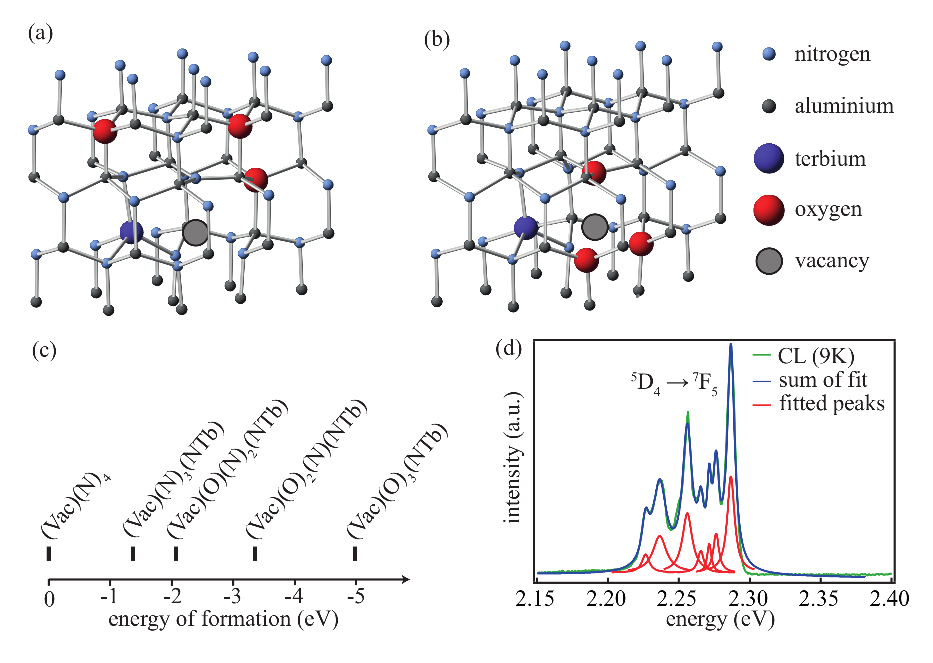
\includegraphics[width=0.5\textwidth]{model}
    \caption{Illustration of the models of the vacancy/Tb$^{3+}$ complex with (a)~no (b)~three oxygen atoms attached to it. (c)~Comparison of the energies of formation of different Tb-N-V$_\text{Al}$ complexes. The names show the four nearest neighbours of the Al vacancy. (d)~High resolution CL spectrum of the $^5$D$_4$ to $^7$F$_5$ transition of Tb$^{3+}$ ions incorporated in AlN.}
    \label{fig:felix_model}
\end{figure}

\section{STEM EELS SI}
\label{sec:STEMEELSSI}
\begin{figure}
	\centering
    
\includegraphics[width=0.5\textwidth]{combined_haadf}
    \caption{(a)~HAADF and maps of (b)~relative thickness, (c)~plasmon peak energy, (d)~plasmon width.}
    \label{fig:combined_haadf}
\end{figure}
All acquired SI have a field of view of $70$~nm and have been rotated through $\sim90^0$ so that the growth direction in all maps points upwards (AlN on top of Si). A HAADF image is shown in Fig.~\ref{fig:combined_haadf}a. The vertical lines in the HAADF image are artefacts due to emission current fluctuations of the cold field emitter electron gun. A relative thickness map is shown in Fig.~\ref{fig:combined_haadf}b. The inelastic mean free path ($\lambda$) values in Si (substrate), AlN:Tb region and SiO$_2$ region at $60$~kV are $\approx49$~nm, $\approx52$~nm and $\approx54$~nm, respectively \cite{egerton2011}. The values of the relative thickness ($t/\lambda$) map can thus be directly related to absolute specimen thickness ($t$) in the range of $13-20$~nm.
\begin{table}%[!ht]
	\caption{Calculated mean free paths ($\lambda$)}.
    \label{tab:lambda}
    \begin{ruledtabular}
    	\begin{tabular}{lccc}
        	Composition&Al:N:Tb:O&Si:O&Si:O										\\
            at.\%&$48:49:2:1$&$33.3:66.7$&$99:1$								\\ \hline
        	$\langle \text{Z} \rangle$&$11.05$&$10.00$&$13.94$					\\
            $\langle \text{A} \rangle$&$23.15$&$20.03$&$27.97$					\\
            $\langle \text{E} \rangle~\left[eV\right]$&$18.0$&$17.4$&$19.6$		\\
           	$\lambda~\left[nm\right]$&$52.4$&$54.0$&$48.9$
    	\end{tabular}
    \end{ruledtabular}
\end{table}
For calculation of $t/\lambda$, the intensity of the spectra up to the minimum between zero-loss peak and plasmon peak is approximated as the intensity of the zero-loss ($I_0$). Hence $I_0$ contains not only zero-loss intensity, but also phonon losses, some retardation and \v{C}erenkov losses etc. The total intensity ($I_t$) also contains inter-band transitions, plasmon losses and ionization core-losses. Hence the $t/\lambda$ values calculated from eqn.~\ref{eq:tl} will always be slight over-estimated (giving a mean of $\overline{t/\lambda}=0.32$ over the whole range in Fig.\ref{fig:combined_haadf}b).
\begin{eqnarray}
	t/\lambda = \operatorname{ln}\left(\frac{I_t}{I_0}\right)
    \label{eq:tl}
\end{eqnarray}
More accurate ways to measure $t/\lambda$ would include fitting the bulk plasmon with a Lorentz function $L(E,E_p,W_p)$ (eqn.~\ref{eq:lorentz}) and the monochromated zero-loss with a Gaussian function $G(E,E_0,W_0)$ (eqn.~\ref{eq:gauss}) and weighting both according to a Poisson distribution $P(n,t/\lambda)$ simultaneously, as shown in eqns.~\ref{eq:poisson} \& \ref{eq:low_loss}.
\begin{eqnarray}
	P(n,t/\lambda) = \left(\frac{t}{\lambda}\right)^n\left(\frac{1}{n!}\right)\operatorname{exp}\left(-\frac{t}{\lambda}\right)
    \label{eq:poisson}\\
	L(E,E_p,W_p) = \frac{A_p}{\pi} \frac{\frac{1}{2}W_p}{(E-E_p)^2+\left(\frac{1}{2}W_p\right)^2}
    \label{eq:lorentz}
\end{eqnarray}
\begin{align}
	G(E,E_0,W_0) = \frac{0.939A_0}{W_0}\operatorname{exp}\left(-\frac{(E-E_0)^2}{0.36W_0^2}\right)
    \label{eq:gauss}
\end{align}
\begin{align}
	S(E,t/\lambda,E_0,W_0,E_p,W_p) = P(0,t/\lambda)~G(E,E_0,W_0) \nonumber \\
     +\sum_{k=1}^{n}P(k,t/\lambda)~L(E,k\times E_p,W_p)    \label{eq:low_loss}
\end{align}
where $n = \lfloor E_{max}/E_p \rfloor \in \mathbb{N}$ is the integer number of plasmon losses considered. $t/\lambda$, position ($E_0$) and full width at half maximum (FWHM) ($W_0$) of the zero-loss peak, position ($E_p$) and FWHM ($W_p$) of bulk plasmon are the fitting parameters. Eqn.~\ref{eq:tl} can be used as an initial estimate of $t/\lambda$ in multiple linear least-squares (MLLS) fitting of the low loss in eqn.~\ref{eq:low_loss}. This can be extended to the entire SI, which provides more accurate $t/\lambda$ values ($\overline{t/\lambda}=0.31,~\overline{\mathbb{R}^2}=0.992$). Figs.~\ref{fig:combined_haadf}c and \ref{fig:combined_haadf}d are maps of $E_p$ and $W_p$ obtained from eqn.~\ref{eq:lorentz} where the values of the plasmon peak energy have been interpolated to sub-pixel precision ($\approx$0.1eV). The FWHM  ($W_p$) of bulk plasmons (Fig.~\ref{fig:combined_haadf}d) of oxides are known to be wider than those of compound semiconductors. Elemental maps are shown in Fig.~\ref{fig:combined_maps}a-\ref{fig:combined_maps}e. The background fitting details are listed in Table~\ref{tab:back_fit_table} along with the integration ranges ($\Delta$). The functions used to fit the background are exponential decay (eqn.~\ref{eq:exp_fun}) or inverse power-law functions (eqn.~\ref{eq:pow_law}).
\begin{eqnarray}
	f(E) =
    \sum^{j=k}_{j=1}
    \left[
    \begin{array}{c}
    	A_1 	\\
        . 		\\
        . 		\\
        A_j 	\\
    \end{array}
    \right]
    \operatorname{exp}\left(-\left[
    \begin{array}{c}
    	r_1 	\\
        . 		\\
        . 		\\
        r_j 	\\
    \end{array}
    \right]E\right)
    \label{eq:exp_fun}
\end{eqnarray}
\begin{eqnarray}
	f(E) = AE^{-r}
    \label{eq:pow_law}
\end{eqnarray}
\begin{table}%[!ht]
	\caption{Background fitting details. All numerical values are in eV.}
    \label{tab:back_fit_table}
    \begin{ruledtabular}
    	\begin{tabular}{lllllll}
    		SI	&edge	 &fit begin&fit end&onset&$\Delta$&fit type 	\\ \hline
            low loss&$Al~L_{2,3}$& $23.8$&$70$&$72.8$&$27.3$&Exp2\footnote{Superposition of two exponential decay functions (eqn.~\ref{eq:exp_fun}).} 		\\
            		&$Si~L_{2,3}$&$41.3$&$98$&$99.4$&$105$&Exp2 			\\ \hline
            high loss&$N~K$&$343.6$&$385.6$&$385.6$&$112$&Pow\footnote{Inverse power-law function (eqn.~\ref{eq:pow_law})} 			\\
                	&$O~K$&$427.6$&$517.2$&$525.6$&$112$&Exp1\footnote{Exponential decay function (eqn.~\ref{eq:exp_fun}).} 			\\
            		&$Tb~M_{4,5}$&$727.2$&$1147.2$&$1211.6$&$246.4$&Exp1 	\\
    	\end{tabular}
    \end{ruledtabular}
\end{table}\\
The value of $k = 1$ for fit type \lq{Exp1}\rq{}, but $k = 2$ for fit types \lq{Exp2}\rq{} and eqn.~\ref{eq:pow_law} for fit type \lq{Pow}\rq{} as indicated in Table~\ref{tab:back_fit_table}. The Si L$_{2,3}$ edge and Al L$_{2,3}$ core-losses are extracted from low loss SI. N K, O K and Tb M$_{4,5}$ edges are extracted from high loss SI. The integration range ($\Delta$) for Al L$_{2,3}$ is limited by overlap with the Si L$_{2,3}$ edge. The maps of Al L$_{2,3}$ and Si L$_{2,3}$ (Fig.~\ref{fig:combined_maps}a \& \ref{fig:combined_maps}b) are relatively noisy due to the low exposure time and hence low signal-to-noise ratio (SNR). Large negative values in the Si L$_{2,3}$ map are due to poor background fitting in the AlN region due to the preceding Al L$_{2,3}$ ionization edge. Deconvolution is not applied because of the low SNR in the spectrum: deconvolution by Fourier-ratio or Richardson-Lucy methods would increase the noise even further. The interface in the high loss maps (Figs.~\ref{fig:combined_maps}c-\ref{fig:combined_maps}e) appears to be inclined w.r.t the horizontal by an angle of $\approx4.6^\circ$ due to drift during the long time of acquisition. Due to this mismatch in the interface, the atomic \% values have been calculated only in the regions indicated in Fig.~\ref{fig:combined_maps}f. The apparent SiO$_2$ layer widths in Fig.~\ref{fig:combined_haadf}d and Fig.~\ref{fig:combined_maps}d differ by 3.5nm due to slight drift between low and high loss region SIs, but this does not prevent direct comparison of Figs.~\ref{fig:combined_maps}c-\ref{fig:combined_maps}e.
\begin{figure}%[!ht]
    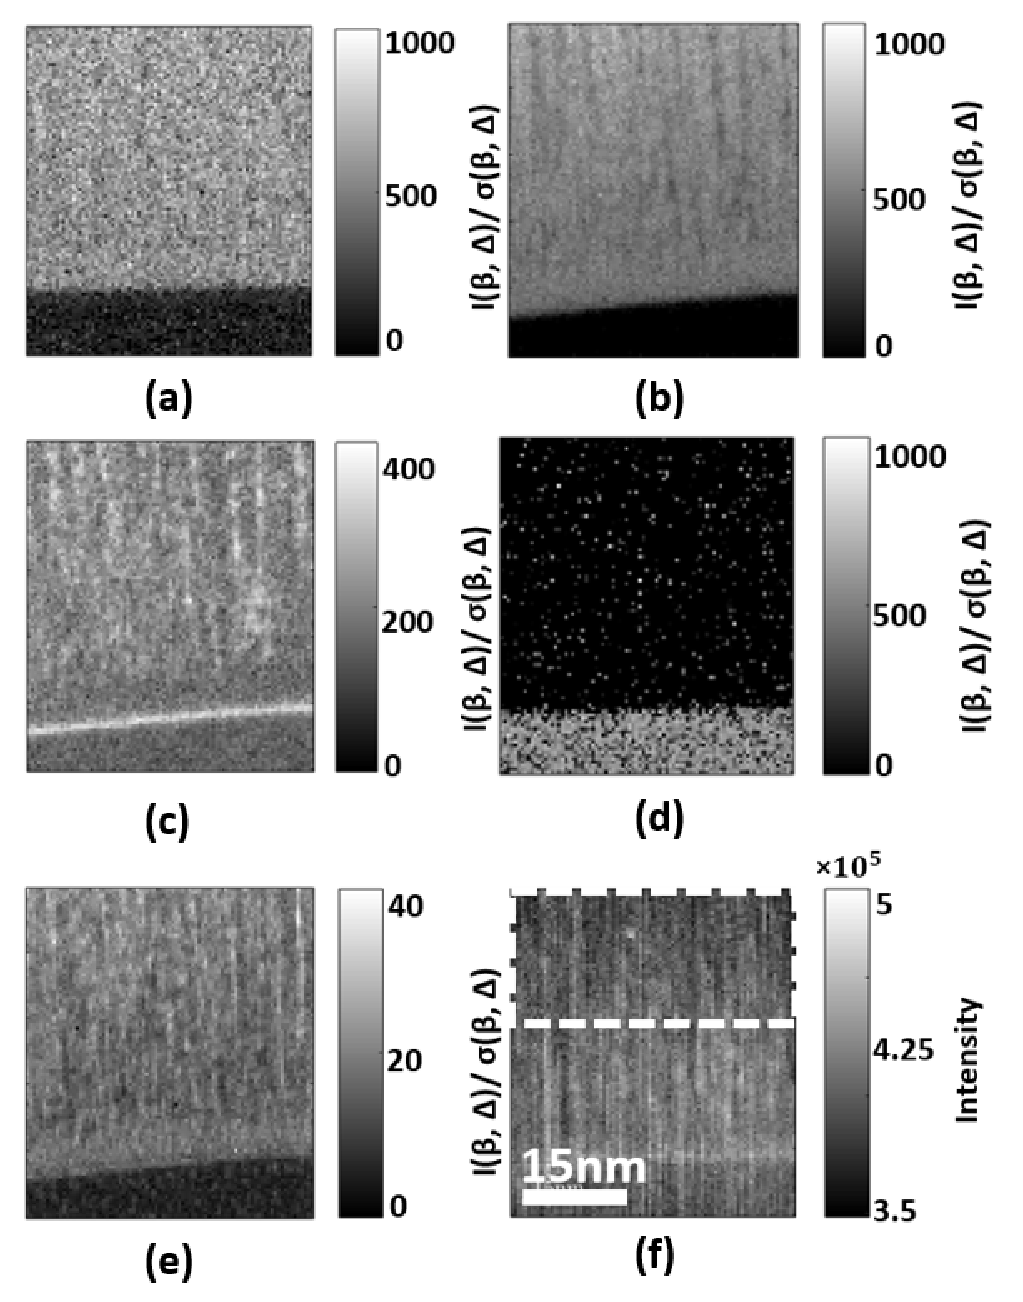
\includegraphics[width=0.5\textwidth]{combined_maps}
    \caption{Background subtracted net intensities after the edge onsets have been integrated and normalised w.r.t the corresponding scattering cross-sections and exposure times. Elemental maps of Al L$_{2,3}$ (a) and Si L$_{2,3}$ (b) in the low loss region. Elemental maps of N K (c), O K (d) and Tb M$_{4,5}$ (e) in the high loss region. (f)~Marked boxes in the AlN region (A) and Si substrate region (B) were used for the calculation of correlation between elemental maps.}
    \label{fig:combined_maps}
\end{figure}
\begin{table}%[!ht]
	\caption{Elemental quantification (at\%) in AlN:Tb and Si region for top 40 rows (A) and lowest 15 rows (B) respectively.}
    \label{tab:atper}
    \begin{ruledtabular}
    	\begin{tabular}{ccccccc}
        	&Region&Al&N&Tb&O&Si						 \\ \hline
            A&AlN:Tb&$43.2$&$38.7$&$1.4$&$15.8$&$0.01$   \\
            B&Si &$17.2$&$0$&$0.8$&$20.3$&$62.3$
    	\end{tabular}
    \end{ruledtabular}
\end{table}
\section{Discussion} %(Anti) correlation of elemental maps
\label{sec:discussion}
In case of N K and O K (Figs.~\ref{fig:combined_maps}b~\&~\ref{fig:combined_maps}c), the contrast of the maps indicates anti-correlation, i.e. in the AlN region, O is replacing N (group V sub-lattice). Tb must be replacing Al in the group III sub-lattice, although the corresponding decrease in local Al contrast is too small to become clearly visible in Fig.~\ref{fig:combined_maps}a. Table~\ref{tab:xcorr} lists the cross-correlation values between the elemental maps in the top half of AlN marked in Fig.~\ref{fig:combined_maps}f. The cross-correlation of N and Tb map is negative. Similar observations can be made between N and O. The cross-correlation between Tb and O maps is positive, indicating the formation of Tb-O complexes. In conclusion, the STEM analysis suggest a co-segregation of the Tb ions together with O ions (which are a common impurity of AlN) in AlN. These experimental results are consistent with atomistic simulations in Fig~\ref{fig:felix_model}b.
\begin{table}[h]
	\caption{Cross-correlation between elemental maps in $AlN$ region marked by box in Fig.~\ref{fig:combined_maps}f}
    \label{tab:xcorr}
    \begin{ruledtabular}
    	\begin{tabular}{cccccccc}
        	$X_{corr}$&Al&N&Tb&O&Si													\\ \hline
            Al& $1.0000$& $0.0802$& $0.0337$& $0.0012$&$-0.0920$					\\
             N& $0.0802$& $1.0000$& $\textbf{-0.0366}$&$\textbf{-0.3694}$&$-0.0060$	\\
            Tb& $0.0337$&$-0.0366$& $1.0000$& $\textbf{0.3466}$&$0.0064$			\\
             O& $0.0012$&$-0.3694$&	$0.3466$& $1.0000$&$0.0188$						\\
            Si&$-0.0920$&$-0.0060$&$0.0064$&$0.0188$& $1.0000$
    	\end{tabular}
    \end{ruledtabular}
\end{table}
\begin{acknowledgments}
We gratefully acknowledge the use of facilities within the LeRoy Eyring Center for Solid State Science at Arizona State University. FB acknowledges the long-standing guidance and help of Prof. Dr. H. P. Strunk who passed away on 17$^\text{th}$ of August 2015.
\end{acknowledgments}

%\nocite{*}
\bibliography{aipsamp}% Produces the bibliography via BibTeX.

\end{document}
%
% ****** End of file aipsamp.tex ******